\newpage
\section{Aufgabe 1: a}

\subsection{Aufgabenstellung}
Machen Sie sich zunächst mit dem Befehl und den Parametern vertraut. Auch der Name Server, der von \texttt{nslookup} angesprochen wird, hat eine IP-Adresse. Wie lautet die Defaultadresse? Wie kann diese verändert werden? (1 Punkt)

\subsection{Vorbereitung}
Um diese Aufgabe lösen zu können, muss man sich mit dem Befehl \texttt{nslookup} auseinandersetzen und herausfinden wie man diesen konfiguriert. 

\subsection{Durchführung}
Die Default Adresse lautet \texttt{192.168.2.1}, also die IP des Routers, und kann mit einer \texttt{nslookup} Abfrage herausgefunden werden. Der erste Eintrag dort ist es, siehe \autoref{nslookup}.

\begin{figure}[H]
	\centering
	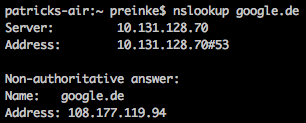
\includegraphics[width=0.4 \linewidth]{images/11}
	\caption{Ausführung von nslookup am Campus Minden} \label{nslookup}
\end{figure}

Um diese Default Adresse zu ändern, schreibt man einfach die DNS-IP die man nehmen möchte hinter die URL, siehe \autoref{newServer}.

\begin{figure}[H]
	\centering
	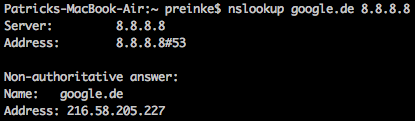
\includegraphics[width=0.4 \linewidth]{images/12}
	\caption{Ausführung von nslookup mit anderem Server}\label{newServer}
\end{figure}

\subsection{Fazit}
Die Aufgabe war nachdem einlesen in das \texttt{nslookup} Kommando, war diese Aufgabe leicht zu lösen.

\newpage
\section{Aufgabe 1: b}

\subsection{Aufgabenstellung}
Bestimmen Sie per Forward-Lookup die IP-Adressen der folgenden Server: (0,5 Punkte)

\begin{itemize} 
\item www.google.com
\item www.spiegel.de
\item whitehouse.gov
\item bundesregierung.de
\item localhost
\end{itemize}

\subsection{Vorbereitung}
Um diese Aufgabe lösen zu können, muss man sich mit nslookup auseinander gesetzt haben

\subsection{Durchführung}
\begin{table}[H]
	\tablestyle
	\begin{tabular}{lll}
		\toprule
			Server & IP-Adresse \tabularnewline
				
		\midrule
			www.google.com & 172.217.21.196 \tabularnewline
			www.spiegel.de & 128.65.210.180 - 128.65.210.185, siehe  \autoref{nslookup:spiegel} \tabularnewline
			whitehouse.gov & 23.211.169.89 \tabularnewline
			bundesregierung.de & 46.243.126.120 \tabularnewline
			localhost & ** server can't find localhost: NXDOMAIN \tabularnewline
			
	\end{tabular}
\end{table}

\begin{figure}[H]
	\centering
	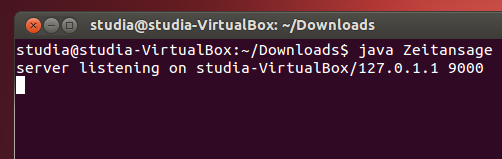
\includegraphics[width=0.4 \linewidth]{images/13}
	\caption{Ausführung von nslookup mit www.spiegel.de} \label{nslookup:spiegel}
\end{figure}

\subsection{Fazit}
Diese war durch die Auseinandersetzung in der vorherigen Aufgabe mit \texttt{nslookup}, sehr leicht zu lösen.

\newpage
\section{Aufgabe 1: c}

\subsection{Aufgabenstellung}
Warum ist die Umrechnung von Host-Namen auf Adressen sinnvoll? (0,5 Punkte)

\subsection{Vorbereitung}
Es gibt keine Vorbereitung auf diese Aufgabe.

\subsection{Durchführung}
Hostnamen sind leichter zu lesen und zu merken für die Menschen als IP-Adressen, für Menschen. Die Benutzer bekommt zum Beispiel auch nicht mit, wenn der Server hinter dem Hostname sich verändert, weil dieser immer der selbe bleibt. \\\\Umgekehrt ist es sinnvoll, damit man nachschauen kann ob sich der Server hinter dem Hostnamen sich geändert hat oder wie viele IP-Adressen überhaupt dort hinter liegen.  

\subsection{Fazit}
Die Aufgabe gibt ein einfaches Grundverständnis über IP-Adressen, die Umrechnung auf Hostnamen und umgekehrt.

\section{Aufgabe 1: d}

\subsection{Aufgabenstellung}
Warum ist bei vielen Web-Servern im Internet ein Reverse Lookup nicht möglich? Auf welcher Art von Servern ist ein Reverse Lookup sinnvoll und i.d.R. auch zwingend erforderlich? (1 Punkt)

\subsection{Vorbereitung}
Um diese Aufgabe lösen zu können, muss man herausfinden was ein Reverse Lookup überhaupt ist.

\subsection{Durchführung}
Ein Reverse Lookup ist quasi das selbe wie ein normaler Lookup, nur gibt man hier die IP-Adresse des Hostnamen an. \\\\Ein Reverse-Lookup funktioniert nur dann, wenn der Server eine sogenannte \texttt{Reverse Lookup Zone} für die IP-Adressen hinterlegt hat. \\\\Ein Reverse Lookup sind dort sinnvoll bei einer Fehlerdiagnose bei Traceroutes. Ein Reverse Lookup ist zwingend erforderlich bei Mailservern, da diese eingehende Mails nur dann akzeptieren, wenn die IP-Adresse des Senders über einen Reverse-DNS-Eintrag verfügt \cite{dns}.

\subsection{Fazit}
Diese Aufgabe war nachdem einlesen in Reverse Lookups, auch relativ leicht zu bewältigen.

